\chapter[SCP-184 建筑师]{
    SCP-184 The Architect\\
    SCP-184 建筑师
}

\label{chap:SCP-184}

\begin{figure}[H]
    \centering
    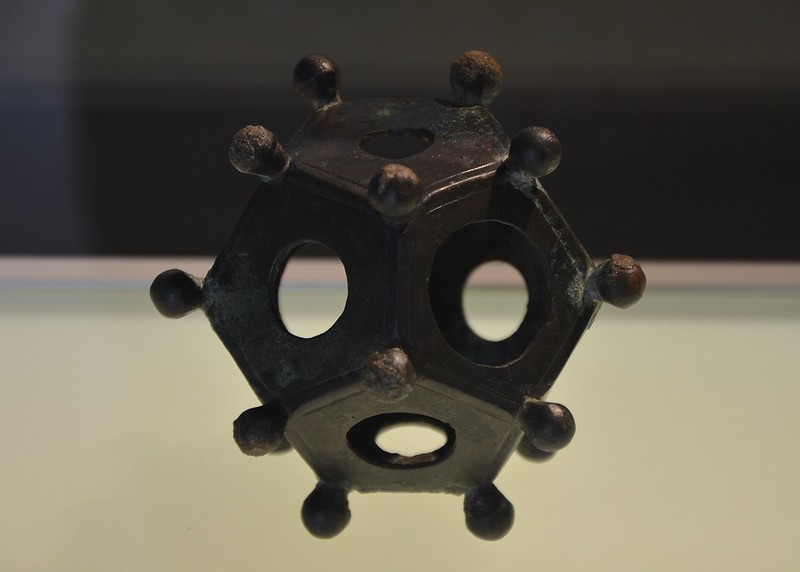
\includegraphics[width=0.5\linewidth]{images/SCP-184.jpg}
    \caption*{SCP-184}
\end{figure}

\bb{项目编号:}SCP-184

\bb{项目等级:}Euclid

\bb{特殊收容措施:}SCP-184不能收容在任何建筑之中。SCP-184在任何时候都要与一个高功率的电磁铁连接在一起。如果该电磁铁失效,特工们要到SCP-184的收容区域进行报道并且防止所有未授权人员的进入直到SCP-184的电磁铁重新通电为止。现阶段SCP-184的收容区域的配置表现为一个公园,其中SCP-184和它的电磁铁伪装成了一座雕塑。对所有参观者进行监控。

所有被SCP-184所影响的建筑都要在被{[}\hyperref[chap:TAIL-code-name-the-truth]{数据删除}]审查之后摧毁,最后进行摧毁的通过权或是归入SCP的决定权也掌握在这人手里。不允许在没有得到许可或是没有救援队在旁待命的情况下进入受影响的建筑进行调查。

\bb{描述:}SCP-184是一个小型的、光滑的金属物体,10cm高4cm宽,表现为正十二面体的外形。这个物体每一个面的中心上都有一个圆形的洞,并且在每一个顶点上都有着一个小球。SCP-184是由一种未知的,但是具有高磁性并且硬度相当于黄铜的合金制成的。

当进入一个封闭的建筑后,SCP-184将会拓展该建筑的内部空间而不改变其外部空间。SCP-184将会以每天数百英尺的速率拓展任何封闭建筑的内部空间,这将会发生在SCP-184进入该建筑一小时之后。最初,SCP-184只是延伸墙的长度,使得该房间变得更大但是并不匹配于该房间的高度。这些将会一直持续直到它变成了它原本体积的3倍大。

到了这一个阶段,SCP-184将会创造出全新的房间。很明显SCP-184可以在该建筑内部复制物体,创造出与该建筑其余房间一致的带家具的房间。但是,在过了一段时间之后,这种拓展加工会开始发生崩坏。例如物体将会由不正确的材料制成(例如玻璃书,木头做的微波炉),房间将会变得奇形怪状,门会对着空白的墙壁开启,并且门廊会变得十分狭窄或者扭曲盘旋变得如同长长的迷宫。这些新的内部结构将会变得越来越奇异,虽然其外观仍然没有改变。

这种行为都大部分地戏剧性地表现在家之中,虽然,这种行为也已经在其他实体之中展现,包括一个硬纸板盒。这种现象并不会随着SCP-184的移除而消失,但是不会有新的结构出现。

\hr

\bb{附录184 - 1:}来自于█████博士的注释

我不认为我必须强调这东西绝对不能在Site-19之中出现。我们必须在某些时刻调查不同的收容站点,但是现阶段,我们必须保持它是露天的、不能移动的又是隐蔽的。

\bb{附录184 – 2:}关注地点

当前假设SCP-184或具有相似性质的异常可能创造了诸如\hyperref[chap:TAIL-alternate-character-interpretations]{苏活区后门}和\hyperref[chap:TAIL-making-a-scene]{山阴山阳地方地下室}\footnote{\bb{译注:}此处原文为“Chūgoku Cellar”,其中“Chūgoku”指日本本州岛西部的一个地区,准确地名翻译为“中国地方”。为了不影响理解此处改用别
称。}等关注地点。有关SCP-184是否是这些空间潜在来源的调查正在进行中

\bb{附录184 – 38RB:}回收记录

SCP-184在████的6月在九龙城寨被发现。关于这个建筑的怪异和爆炸式的增长的报告吸引了操作员,他们不久之后就发现了SCP-184。被{[}数据删除]所掌握。在数次警察镇压之后,机动特遣队Zeta-9被派遣到现场并以最小的代价获得了SCP-184。因为当地强制法律执行行为的妄动,SCP-184暴露在该城寨和居民之下的最后效果将永远不能被理解了,在操作员采取措施阻止他们之前他们摧毁了数个受影响的区域。

对于获得最少信息的居民的采访之中,一个公社的“沉默之墙”成为了最主要的回答。一些文档提到SCP-184可以被带入家庭之中并且以每半小时50英磅的价格让它影响其寓所。这些文档没有得到当地居民的确认。

\bb{附录184 – 38RB-s:}附加文档

\hyperref[sec:DOC-personal-log-of-gordon-richards]{Gordon Richards的个人日志} — 一名机动特遣队Zeta-9“鼹鼠”(the Mole Rats)的队员

\newpage
\section{Gordon Richards的个人日志}

\label{sec:DOC-personal-log-of-gordon-richards}

\begin{figure}[H]
    \centering
    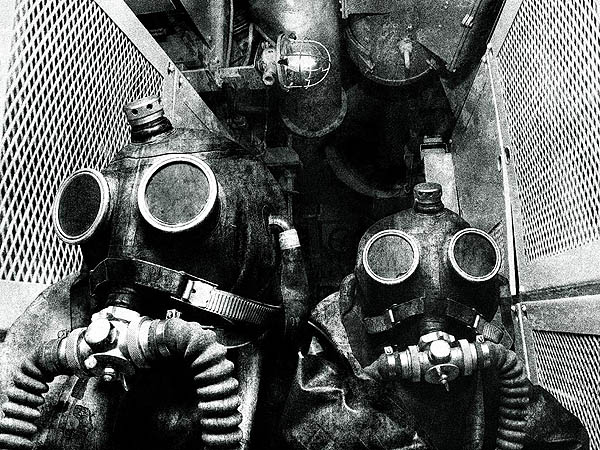
\includegraphics[width=0.5\linewidth]{images/personal-log-of-gordon-richards.jpg}
    \caption*{Gordon Richards 与 Lev Shattaerman在九龙城寨下的下水道中}
\end{figure}

\bb{个人日志归属:}Gordon Richards,机动特遣队Zeta-9,“鼹鼠”成员

\bb{日期:}3\slash 6\slash ████

被派遣到“九龙城寨”去获得一个物体,并且对其所影响的东西都建立文档。我从没有见过这么可怕的一个地方,四处都是秽物,整面的墙甚至整栋建筑物都是由垃圾建成的。如果你松开你的套装哪怕只是1秒钟,你将会被烟草、油烟、汗臭、机油和粪便的味道淹没。Henry在穿过了一条满是垃圾的过道之后掉进了一个在地上作为下水道的坑中。他还好,他的衣服只是脏了,但是他呕吐不止并且只能被带走了。我不知道他能不能解决这个问题。

这里的每个人都像躲避瘟疫那样躲着我们,或是走出来向我们扔垃圾和辱骂我们。他们是一个部落,并且是十分有着领土意识的部落。这里的人口密度高的吓人,并且我很庆幸在我和他们之间还隔着制服。那东西应该是在这个地方的核心处,但是想要穿过这里真是棘手不堪。

\hr

\bb{日期:}4\slash 6\slash ████

当地的执法部门在特工的引领下昨晚发起了一次进攻。他们把人从我们将进入的某些区域驱赶了出来,但是这里实在有太多的人了以至于这实在没让人觉得有什么不同。昨天侦察队帮我们发现了好几个被那东西影响了的“家宅”。它们看起来不像那些已经司空见惯了的、肮脏的住宅,但是它们内部实在是太大了。这是一种古怪的感觉,把你的手放在墙上站着,知道从任何方面来说你呆着的这建筑外面空间上只有6平方英尺大。Henry今天好些了,但是看起来实在是有点神经质。Lev昨晚把他带到一边并且和他谈了谈,我希望这能有点效果。我现在开始有些担心他了,因为今天我看到了他在对着电台自言自语。我让他闭嘴,但是我没有把这件事情报告上去,或许我真应该这样做的。我想我应该在这次任务结束之后申请把他调到另一个单元去。

夜晚进行了深入的侦察,我们分开来以尝试找到那东西隐藏的地点。Lev和我都撑着一根短棍并且凭借这东西在下水道系统内部巡游。诚实地说,再没有什么能比上面更糟的了,至少在这里我们不用一直面对那些人面无表情的脸。

\hr

\bb{日期:}6\slash 6\slash ████

Henry死了。我们在今天早晨凌晨时分才回来;因为干扰,我们已经好几个小时没有用电台联系了。看起来这地方受那东西的影响使得无线电波被严重地扭曲了。那些下水道就是噩梦,但是没有发现被那东西扭曲的迹象。当我们回来了之后,Paul告诉了我们最新消息,Henry和Paul在这城市中心附近进行探索,就是在那时他们遭到了攻击。一大群暴徒把他们包围了并且把Henry拖走了。Paul受伤了并且他的制服也严重损坏了,而且他不得不撤离以接受治疗。Henry在电台频道里尖叫了一阵之后声音被掐断了。Paul和其他特工一起想要去救出Henry,但是在几分钟之后,Henry重新出现在了电台频道里。

他的接收器损坏了,但是他仍然能够广播。一名特工进行了记录,然后他把记录对Lev和我重播了一遍,以看看其中是否有什么内容是对我们有意义的。但是那其实一点意义都没有,他在漫无边际地说这话,听起来他似乎受伤了。一直再说着这城市永无止尽的中心,玻璃构成的地狱,所有能使人发狂的东西。Paul和援救队伍一直在寻找他,但是再一次地他的无线电信号又被掐断了。

Henry撕开了一个小小的房间并冲了出来,头盔掉了并且像个疯子一样尖叫着。他正好从Paul的身边跑过并且将一名前去找他的特工砸进了墙里。他最终撞死了并且就在那之后爆炸了,就在建筑的外面。他的六块身体碎片掉在了一些垃圾上。清理他的碎片花了我们一个小时的时间。我们在这里所做的一切都扭曲了,Parks特工、Lev和我聚集了这城市里的所有长者,然后我们马上就会到达这该死的一切的终点了。

\hr

\bb{日期:}7\slash 6\slash ████

审问进行得很顺利。Parks特工问问题,我们则处理那些他叫做“不合作者的负面回答”的东西。那第一个家伙,一些傻×朋克青年,不想开口。在打断了他两条腿之后,他变得合作多了,提到了某些东西使他们成为“建筑师”的。没有人知道它是什么时候来到这个城市里的。他从来没有用那东西做过任何事情,只是在那东西工作时负责在门口看守。他说那就是他知道的全部了,如果我们想要知道它是什么,我们就必须和一名长者,Long-Wen谈谈。他为Henry的死道歉,说那是自然发生的事情,我打碎了他下巴的三处地方。

Long-Wen有可能是我见过的最老的人了,并且有着钢铁般的意志力。他经受住了我们的所有折磨,一声也不吭。Parks威胁他如果他再不说就要在他的妻子儿女身上进行折磨了,而这让他开了口。他告诉我们那东西被保存在这座城市最古老的一个区域之中,一些古老的神庙里。它们在成长,并且会创造出难以置信的东西来,但是只有配得上那东西的人才能亲眼看到它而不被它打垮。他说Henry已经看到过那些奇迹了,他们希望Henry说服我们不要带走“建筑师”,但是他不是能配得上它的人,所以他崩溃了。

我们迫使他带我们去看保存那东西的地方。Long-Wen说那不会有好结果的,因为那已经被埋藏得太深了。他们在一看见特工出现时就已经那东西深深地藏了起来;他还说我们永远都不可能带回那东西的。看来明天我们要做一些“深度工作”,我们不会在没找到那东西之前出来的。

\hr

\bb{日期:}10\slash 6\slash ████

我们失神了一会儿,这里实在是太令人震惊了。一开始,那只是一个内部大到不可思议的神庙,整洁但是没有什么东西是新的。接着我们往下走,所有的房间,祭坛,所有的东西都被复制了并且都是由这些东西反复构成的。就像是有个人在这个狭小的庙宇空间里面建造了12个一模一样的神庙。Parks特工在主墙上放了一个召回点,其他特工在确保没有人跟踪我们。我们穿好了装备并且开始工作了。六个小时之后,一切看起来都变得古怪了。成堆的门廊,变少了的房间,83个都由滑门连接的房间,每一个都在房间中央有着一个小小的佛像,而在没有其他东西了。Lev收集了一些样品。当我们进入一个与第一个房间相同完美的复制品,但是其中更多的东西是由木头制成的房间时,我们知道事情将会变得越来越怪异了。

每一件东西都是精美的而天衣无缝的,甚至在所有的东西上都没有工具的痕迹。Paul发现了一些文档,我扫描了它们并且把他们传回给了Parks。他说这是有关于那东西的文档,很明显我们现在把它称作SCP-184了,Parks说这些文档上提到在184创造出一个新的区域时,他们就把184带到更深的地方。他们认为这是来自于神或是其他什么东西的礼物,并用它来拓展房间,如果人们向寺庙捐献,或是至少向现在控制着这东西的帮派捐献的话。

我从来就没有到过像这样的一个地方,这里越来越难以行进了,墙壁开始变得奇怪了,它们开始向上以有趣的角度延伸,最后的几个房间都已经变得极为狭小了。根据Lev的计算,我们已经在城市上方大约20英尺的地方了。

\hr

\bb{日期:}12(?)\slash 6\slash ████

我已经对这地方感到恶心了,昨天我们来到了一个岔路口,不得不将队伍分开。我选择了“向上”的门廊,并且出发了。我不能确定我们已经爬了多高,墙壁已经不像之前那么规律了。它们像波浪一样左拐右拐,就像一场被凝固了的地震。看起来这里的所有东西都是用石头做成的。我成功地挤进了旁边一个房间来喘口气,环顾四周时,我发现所有的东西都是由碧玉雕成的。它们都被上了正确的颜色,有着一致的纹理,但是它们都是由玉做成的。床、椅子、书桌、书,所有的一切。我坐在那玉床上2个小时,什么都不想。之后我站了起来并砸碎了那个可能比我的命还值钱的玉台灯,之后离开了这里。

我的感觉很糟,在这里我就像与世界切断了联系,像是宇航员或者其他的什么东西。这里不像我曾经到过的那些区域。从未感觉如此孤独。我很好,我知道的。Henry死了,死在外面那整个都在腐烂的城市里,但我是孤独的并且什么都没办法去想。老鼠们能被测试心理稳定性,而我只是在这些飞窜而过的色彩之中不停地行进着。那只是我神经紧张罢了,我正坐在由一千条小龙雕像构成的椅子上,正在一张由超高密度的纸形成的桌子上写字,我很好。

\hr

\bb{日期:}(?)\slash 6

我已经出来得太久了,食物短缺,饮水短缺。但是都还没有耗尽,但我还是在这里,听着东西,一直想着我在听某些东西。已经攀爬了好几天,今天看到了光。在一个旁厅的尽头,明亮的黄光,我爬进了那厅里之后跑了起来,直到撞开了门,那里面是一个房间,放着数以百万计的蜡烛,都点亮了,但是这仅仅只是另一个房间而已。我脱下了我的头盔,用它把这些蜡烛都狠狠地砸碎了。我打坏了我的透镜、我的护膝、我的电台,这都不重要了。坐下来哭了好几个小时。今天我在一根杆子上绑了一些东西然后将它扔了下去,根本就没有听到它触底的声音,我差点就想跳下去把它捡回来,但是我最终还是忍住了。去找到那东西,去把它砸成碎片,跺烂它,粉碎它。

\hr

\bb{日期:}(?)\slash 6

食物吃完了,套装之中也再不能产生水了,看到了一堵有着一万道门的墙壁,我从那下面跑过,打碎了一连串的门,然后接着爬。我的靴子丢了。地板看起来就像地毯一样。但是是由极度锋利的石头组成的,它们把我的衣服切成了布条,同样的遭遇也发生在我的脚上。血洒在了通道上,希望它能够喜欢。去打碎这些东西。觉得在我心里有什么东西破碎了。我一直听到Henry的声音,我一直告诉他他已经死了,但他都不听。

\hr

\bb{日期:}(?)

通道的顶端、永无止尽的大厅、无处不在的光。走啊走啊直到心也碎裂。

\hr

\bb{日期:}(?)

天堂就是地狱\\
地狱就是天堂\\
生命如此美好

\hr

\bb{注释:}Gordon Richards在获取SCP-184的行动之中走失了,推断为KIA,SCP-184被Zeta-9成功获取,就在被摧毁的被SCP-184所影响的神庙的碎石堆之中发现了。

